\label{capitolo4}
\section{Modelli e problemi di controllo}
Nel controllo di sistemi elettrici possiamo incontrare due tipi di problemi:
\begin{itemize}
\item \textbf{problemi di controllo di potenza} nei quali si cerca di fornire la potenza richiesta agli utilizzatori; minimizzando i costi globalmente o fornendo la massima potenza richiesta minimizzando i costi del singolo generatore.
\item \textbf{problemi di controllo di energia} nei quali si richiede che l'elettricit� abbia voltaggio e frequenza necessari per cooperare con tutti i generatori e i carichi. 
\end{itemize}
Questi problemi sono apparentemente interlacciati in quanto dipendono entrambi dai generatori. Inoltre, solo ai generatori si applicano i meccanismi di controllo mentre i carichi sono considerati disturbi esogeni.\\
Possiamo considerare due tipi di generatori, il primo con masse rotanti e alternatori, il secondo senza masse rotanti ma con inverter.
I generatori con masse rotanti forniscono la potenza richiesta aumentando o diminuedo la velocit� di rotazione con conseguente alterazione della frequenza.\\
Quando ci spostiamo dal controllo dei generatori al controllo del carico della rete incontriamo un secondo problema ovvero il problema del flusso di carico; infatti si vuole distribuire la potenza senza per� sovraccaricare le linee e possibilmente minimizzando le perdite di carico.\\
\subsection{Modello di un generatore termoelettrico}
Questo tipo di generatore � formato da una massa rotante nel quale potenza e frequenza sono accoppiate.\\
Prendiamo il caso di un generatore isolato nel quale abbiamo una fornace nella quale si brucia del carburante e di conseguenza si produce calore, il calore prodotto trasforma un fluido in vapore, questo vapore fa muovere una turbina che infine fa muovere l'alternatore.\\
Prendiamo in considerazione come ingresso il sistema che brucia carburante e come uscita la potenza meccanica dell'alternatore. Per semplicit� consideriamo come ingresso esogeno la potenza $P_c$ prodotta dalla combustione e rilasciata al contenitore principale di energia (vapore).
Il bilancio di energia immagazzinata � dato da:
$$\dot{E}= P_c-P_{loss}-P_t$$
dove $P_{loss}$ � la potenza persa nelle pareti esterne mentre $P_t$ � la potenza consumata dalla turbina.
Per semplicit� assumiamo che l'immagazzinatore di energia sia completamente vapore e che la sua massa sia costante; a questo punto possiamo associare la $P_{loss}$ alla differenza di temperatura tra la temperatura di saturazione del vapore a una certa pressione $p$ e la temperatura esterna tramite la relazione:
$$P_{lost}=G_{loss}(T_{sat}(p)-T_{ext})$$
In generale la $T_{sat}>>T_{ext}$ cos� possiamo scrivere che:
$$P_{loss}=K_{loss}\frac{E}{M}$$
dove $K_{loss}$ � un opportuno parametro legato alla superficie di dispersione, e la divisione per $M$ esprime la dipendenza della potenza dallo stato del vapore.\\
Un'altra semplificazione riguarda $P_t$ infatti trascuriamo il surriscaldamento che subisce il vapore all'atto dell'attraversamento della turbina e facciamo dipendere $P_t$ soltanto dalla pressione ($E/M$) e dall'apertura della valvola della turbina $\theta \in [0,1]$
$$P_t=\theta K_{draw} \frac{E}{M}$$
e dove $K_{draw}$ � un altro parametro.\\
La potenza meccanica che raggiunge l'alternatore � ottenuta tenendo conto dell'efficenza meccanica dell'alternatore assunta costante e chiamata $\eta_m$
$$P_m=\eta_m P_t$$
Mettendo le equazioni a sistema otteniamo
\begin{equation}
\left\{
\begin{array}{ccccc}
\dot{E}&=&P_c-K_{loss}E/M&-&\theta K_{draw}E/M\\
\\
P_m&=&\eta_m\theta K_{draw}E/M&&
\end{array}
\right.
\end{equation}
Sapendo che $[K_{loss}E/M]=[K_{draw}E/M]=[W]$ e $\theta$ e $\eta_m$ sono adimensionali ricaviamo che $[K_{loss}/M]=[K_{draw}/M]=[1/s]$ e possiamo riscrivere il sistema precedente come:
\begin{equation}
\left\{
\begin{array}{ccccc}
\dot{E}&=&P_c-\big(\frac{1}{T_{loss}}&+&\frac{\theta}{T_{draw}}\big)E\\
\\
P_m&=&\frac{\eta_m}{T_{draw}}E\theta &&
\end{array}
\right.
\end{equation}
In questo caso $T_{loss}$ e $T_{draw}$ sono le costanti di tempo con le quali l'energia viene rispettivamente persa dalla superficie esterna e prodotta attraverso l'alternatore alla massima apertura della valvola della turbina.
Questo modello risulta molto impreciso e in un caso reale sarebbe applicabile solo nell'intorno di un punto di lavoro. Ma per i nostri scopi � pi� che sufficente.\\
Introduciamo ora la potenza nominale del generatore $P_n$ e chiamiamo $T_{rest}$ il tempo richiesto dal generatore per immagazzinare la sua "energia nominale" definita come $E_n=P_nT_{rest}$. Dividiamo ora entrambe le equazioni per $E_n$
\begin{equation}
\left\{
\begin{array}{ccccccc}
\dot{e}&=&\frac{1}{T_{rest}}p_c&-&\big(\frac{1}{T_{loss}}&+&\frac{\theta}{T_{draw}}\big)e\\
\\
p_m&=&\eta_m\frac{T_{rest}}{T_{draw}}e\theta&&&&
\end{array}
\right.
\end{equation}
Dove $p_c=P_c/P_n$ e $p_m= P_m/P_n$ sono rispettivamente la potenza normalizzata di combustione e meccanica, ed $e=E/E_n$ � l'energia normalizzata.\\
A questo punto calcoliamo l'equilibrio di questo modello per ingressi costanti $\overline{p_c},\overline{\theta}$
$$\overline{e}=\frac{T_{draw}T_{loss}\overline{p_c}}{T_{ress}(T_{draw}+T_{loss}\overline{theta})}$$
$$\overline{p_m}=\frac{\eta_mT_{loss}\overline{p_c}\overline{\theta}}{T_{draw}+T_{loss}\overline{\theta}}$$
A questo punto linearizziamo il modello nelle vicinanze dell'equilibrio imponendo $\Delta p=p_c-\overline{p_c}, \Delta\theta=\theta-\overline{\theta}$ e $\Delta e = e- \overline{e}, \Delta p_m =p_m-\overline{p_m}$
$$
\left\{
\begin{array}{ccccc}
\Delta\dot{e}&=&-\left(\frac{1}{T_{loss}}+\frac{\overline{\theta}}{T_{draw}}\right)\Delta e&+&\left[\frac{p_c T_{loss}}{T_{rest}(T_{draw}+T_{loss}\overline{\theta})}\frac{1}{T_{rest}}\right]\left[\begin{array}
{c}
\Delta\theta\\
\Delta p_c
\end{array}\right]\\
\\
\left[
\begin{array}{c}
\Delta p_m\\
\Delta e
\end{array}\right] 
& = &
\left[
\begin{array}{c}
\frac{\eta_mT_{rest}\theta}{T_{draw}}\\
1
\end{array}\right]
\Delta e &+&
\left[ 
\begin{array}{cc}
\frac{\eta_mT_{loss}\overline{p_c}}{T_{draw}+T_{loss}\overline{\theta}} & 0 \\
0 & 0
\end{array}\right]\left[
\begin{array}{c}
\Delta\theta\\
\Delta p_c
\end{array}\right]
\end{array}
\right.
$$
La corrispondente matrice di trasferimento �:
$$
\begin{array}{lc}
\Gamma(s) &=\left[\begin{array}{cc}
\Gamma_{\theta_m}(s) & \Gamma_{c_m}(s)\\
\Gamma_{\theta_e}(s) & \Gamma_{c_e}(s)
\end{array}\right]=\left[\begin{array}{cc}
\frac{\Delta p_m(s)}{\Delta\theta(s)} & \frac{\Delta p_m(s)}{\Delta p_c(s)}\\
\frac{\Delta e(s)}{\Delta\theta(s)} & \frac{\Delta e(s)}{\Delta p_c(s)}
\end{array}\right]\\
\\
\dots &= \frac{1}{1+s\frac{T_{draw}T_{loss}}{T_{draw}+T_{loss}\overline{\theta}}}
\left[
\begin{array}{cc}
\frac{\eta_m T_{draw}T_{loss}\overline{p_c}}{(T_{draw}+T_{loss}\overline{\theta})^2}(1+sT_{loss})&
\frac{\eta_mT_{loss}\overline{\theta}}{T_{draw}+T_{loss}\overline{\theta}}\\
\frac{T_{draw}T^2_{loss}\overline{p_c}}{T_{rest}(T_{draw}+T_{loss}\overline{\theta})^2} & 
\frac{T_{draw}T_{loss}}{T_{rest}(T_{draw}+T_{loss}\overline{\theta})}\\
\end{array}
\right]
\end{array}
$$
Alcune altre semplificazioni che faremo a livello di sistema per valutare i costi sono:
\begin{itemize}
\item Assumeremo che i costi siano dati solo dal consumo di carburante e non dal mantenimento dell'impianto
\item La combustione non avviene allo stesso modo ai diversi carichi di sistema
\item Il cunsumo specifico $c_s$� definito tipicamente decrescente rispetto a $P_c$.
\item Il flusso di carburante consumato $w_c$ e $p_c$ sono legati dall'equazione
$$w_c=c_s(p_cP_n)p_cP_n;$$
\end{itemize}
La potenza attiva richiesta dal carico, un parametro esogeno per il generatore, viene detta $P_e$ cos� il bilancio delle energie per la massa in rotazione �:
$$J\omega\dot{\omega}=P_m-P_e$$
dove $J$ � l'inerzia totale vista all'albero del generatore (si pensi al caso di pi� generatori).
L'equazione del rendimento all'equilibrio  per ogni $\omega$ e $\overline{P_m}$ e $\overline{P_e}$ siano costanti e coincidenti la linearizazione diventa:
$$\Delta\dot{\omega}=-\frac{P_m-P_e}{J\overline{\omega}^2}\Delta\omega+\frac{1}{J\overline{\omega}}(\Delta P_m-\Delta P_e)$$
Visto che $P_e=P_m$ e che $\omega$ viene regolato al valore desiderato $\omega_0$ otteniamo:
$$\Delta\dot{\omega}=\frac{1}{J\omega_0}(\Delta P_m-\Delta P_e)$$
Normalizzando $P_{m,e}$ con $P_n$ e $\omega$ con $\omega_0$ e usando $\delta$ per indicare le variazioni delle quantit� normalizzate otteniamo:
$$\frac{\Delta\dot{\omega}}{\omega_0P_n}=\frac{1}{J\omega_0}(\frac{\Delta P_m}{\omega_0P_n}-\frac{\Delta P_e}{\omega_0P_n})$$
$$\delta\dot{\omega}=\frac{1}{J\omega_0^2}(\delta P_m-\delta P_e)$$

\subsection{Controllo di un generatore}
Dopo aver descritto la relazione che lega $(\Delta\omega, \Delta p_c)\rightarrow(\Delta p_m, \Delta e)$ e la matrice di trasferimento del primo ordine $\Gamma (s)$. Ricordando inoltre che il contenuto di energia � legato alla pressione del vapore $p$.
Ora parleremo del controllo di pressione nel generatore che significa anche controllare l'energia contenuta nel generatore.\\
Per effettuare questo controllo il nostro problema diventa come controllare la potenza meccanica in uscita dall'alternatore. Per applicare questo controllo si utilizzano principalmente tre metodi:
\begin{itemize}
\item \textbf{boiler follows}: consiste nella modulazione di $\theta$ oer modulare $\Delta P_m$ e $\Delta P_c$ per mantenere costante la pressione; questo permette una regolazione di $P_m$ molto rapida ma che provoca piccole variazioni di pressione che causano un forte stress al sistema.
\item \textbf{turbine follows} consiste nell'usare $\omega$ e $P_c$ per regolare il sistema; con questo metodo si ha un controllo sulla pressione migliore ma il tempo di risposta del sistema � pi� lento.
\item \textbf{sliding pressure} In questo sistema si mantiene $\theta$ al suo valore massimo e si controlla $P_m$ agendo su $w_c$; questo sistema permette di non sollecitare troppo la turbina ma come contro ha dei tempi di risposta molto lunghi.

\end{itemize}

Descriviamo ora gli attuatori che controllano $\theta$ e $P_c$ tenendo conto dei loro tempi di risposta che non sono sicuramente immediati. La matrice di trasferimento �:
$$A(s)=\left[\begin{array}{cc}
\frac{1}{1+sT_{\theta}} & 0\\
\\
0 & \frac{1}{1+sT_{P_c}}\\
\end{array}\right]$$
Quindi in accordo con le dinamiche degli attuatori:
$$\left[\begin{array}{c}
\Delta\theta(s)\\
\Delta P_c(s)
\end{array}\right]=A(s)\left[\begin{array}{c}
\Delta\theta_c(s)\\
\Delta P_{cc}(s)
\end{array}\right]$$
Dove $\theta_c$ e $P_{cc}$ sono le variabili di comando degli attuatori rispettivamente di $\theta$ e $P_c$
Il sistema � cos� modellizzato dalla matrice di trasferimento $\Gamma(s)A(s)$\\
D'ora in poi non indicheremo pi� il pedice "c" per indicare le variabili di controllo e considereremo A(s) come parte del processo, ovvero considerando sempre la cascata tra $A$ e $\Gamma$ ma prendendo come ingressi $\theta$ e $P_c$. In altre parole possiamo scrivere il sistema come:
$$
\left[\begin{array}{c}
\Delta P_m(s)\\ \Delta e(s)
\end{array}\right] 
= \Gamma_{ap}(s)
\left[\begin{array}{c}
\Delta\theta(s)\\ \Delta P_c(s)
\end{array}\right]
$$
dove $\Gamma_{ap}(s)=\Gamma(s)A(s)$\\

Tornando allo scopo principale, il tipo di politica di controllo utilizzata per controllare il sistema si basa su quali tipi di generatori vengono utilizzati, sulle regole della rete e talvolta anche in base al carico presente in quell'istante.
Qualsiasi sia la politica di controllo scelta e qualsiasi sia la variabile di controllo usata per governare $P_m$ (d'ora in poi denotata con $u_P$) il sistema pu� essere controllato dalla funzione di trasferimento $G(s)$ espressa come:
$$G(s)= \frac{\Delta P_m(s)}{\Delta u_P(s)}\Bigg|_{struttura_-generatore,politica_-di_- controllo}$$

Possiamo normalizzare $G(s)$ sostituendo la potenza normalizzata $P_n$ e la variabile di controllo normalizzata $u_{P_n}$ ottenendo:
$$g(s)=\frac{\delta P_m(s)}{\delta u_p(s)}$$
dove $u_{P_n}$ � 1 o $P_n$ se la variabile di controllo � rispettivamente o $\theta$ o $P_c$ in ogni caso lo schema da controllare risulta essere (per un generatore isolato):
\begin{figure}[htb]
\centering
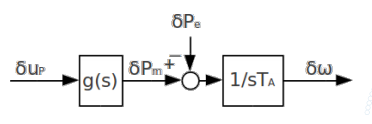
\includegraphics[width=10cm]{img/geniso.png}
\caption{Schema a blocchi di un generatore isolato}
\label{fig:geniso}
\end{figure}
Per il caso di generatore isolato il sistema di controllo risulta essere quello in figura \ref{fig:gencontrol}
\begin{figure}[htb]
\centering
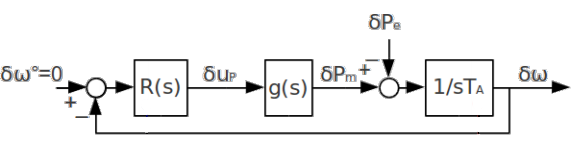
\includegraphics[width=10cm]{img/gencontrol.png}
\caption{Schema del sistema di controllo per un generatore isolato}
\label{fig:gencontrol}
\end{figure}
Dove $1/sT_A$ � un integratore che impone a zero l'uscita in caso di sistema all'equilibrio, mentre $R(s)$ � un altro integratore per mantenere a zero l'errore di frequnza nel caso di sistema all'equilibrio.
\subsection{Generatori in rete}
Prima di parlare del caso di pi� generatori connessi in rete dobbiamo fare alcune ipotesi sulla rete stessa; infatti si suppone che la rete sia rigida e sincrona. I generatori invece ruotano alla stessa velocit� senza drift sul valore impostato.
In questo caso tutta la potenza meccanica (non normalizzata) viene sommata, mentre un unica potenza elettrica viene sottratta (il totale del carico). Il sistema sotto controllo � rappresentato in figura \ref{fig:gennetwork}
\begin{figure}[htb]
\centering
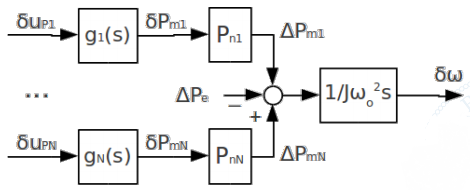
\includegraphics[width=10cm]{img/gennetwork.png}
\caption{Sistema di pi� generatori collegati alla 
rete.}
\label{fig:gennetwork}
\end{figure}
Dove $J$ � l'inerzia totale della rete.\\
A questo punto � facile estendere lo schema del generatore isolato allo scema con pi� generatori come vediamo in figura \ref{fig:netcontrol}.
\begin{figure}[htb]
\centering
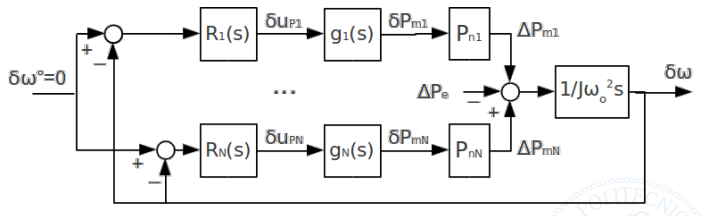
\includegraphics[width=10cm]{img/netcontrol.png}
\caption{Schema del sistema di controllo per un generatore isolato}
\label{fig:netcontrol}
\end{figure}
In questo schema l'integratore ($1/J\omega_0^2s$) garantisce che l'errore sulla potenza in caso di equilibrio sia zero. Mentre i regolatori ($R_1\dots R_n$) non possono essere tutti degli integratori altrimenti avremo delle parti non controllabili del sistema.\\
Per capire il perch� osserviamo lo schema di figura \ref{fig:schema} equivalente al sistema.
\begin{figure}[htb]
\centering
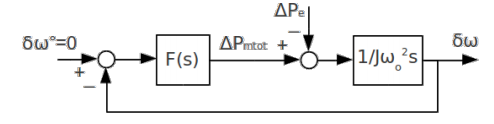
\includegraphics[width=10cm]{img/schema.png}
\caption{Schema equivalente}
\label{fig:schema}
\end{figure} 
Dove $\Delta P_{mtot}$ � la variazione della potenza meccanica totale, e
$$F(s)=\sum_{i=1}^N R_i(s)g_i(s)P_{ni}$$
Degli integratori in $R_i$ andrebbero in parallelo e farebbero perdere la controllabilit�.\\
La soluzione a questo problema � avere un solo integratore:
\begin{itemize}
\item avere un primo regolatore $R_i(s)$ di tipo proporzionale.
\item introdurre un controllore in seconda frequenza di tipo integrale per l'intera rete.
\item l'output del secondo regolatore entra in alcuni correttori che entrano a loro volta nell'ingresso degli $R_i$
\end{itemize}
\section{Applicazione del paradigma OO al modello del generatore}
Fino ad ora abbiamo utilizzato un approccio orientato ai blocchi per descrivere il nostro sistema; ora per� diviene pi� utile descrivere tale sistema con un modello orientato agli oggetti.\\
A questo scopo, come prima cosa definiamo un connettore che esprima l'accoppiamento sincrono e rigido, ovvero nel quale tutti i modelli connessi hanno la stessa frequenza e non presentano fenomeni di disallineamento.
\begin{verbatim}
connector PowerFreqPort
		  Real f; // Frequency
	flow Real P; // Power
end PowerFreqPort;
\end{verbatim}
Definiamo una rete nella quale potremmo collegare diversi generatori ma che controlla una singola inerzia globale.
\begin{verbatim}
model ElectricNetworkPF
	signalIn Pe; // Electric power (exogenous)
	PowerFreqPort Pg; // Port to connect all generators
	parameter Real J = 1000; // Inertia
	parameter Real fo = 50; // Nominal (and initial) frequency
	Real f(start = fo); // Frequency
equation
	der(f) = (Pg.P-Pe)/(J*8*3.14^3*fo^2); // der(2*pi*f)=(Pg-Pe)/(J*(2*pi*fo)^2)
	f = Pg.f;
end ElectricNetworkPF;
\end{verbatim}
Ed infine definiamo il modello del generatore:
\begin{verbatim}
model SimpleThermoElecGenPF
	signalIn 		theta; // Throttling valve command
	signalIn 		Pc; // Combustion power command
	PowerFreqPort  Pg; // Port to network
	parameter Real Pn = 100;
	parameter Real Trest = 500;
	parameter Real Tdraw = 500;
	parameter Real Tloss = 1e9;
	parameter Real etam = 0.95;
	parameter Real thetabar = 0.8;
	parameter Real pcbar = 0.8;
	Real e(start=Tdraw*Tloss*pcbar/Trest/(Tdraw+Tloss*thetabar));
	Real pc,pm;
equation
	der(e) = pc/Trest-(1/Tloss+theta/Tdraw)*e;
	pm = etam*e*theta;
	pc = Pc/Pn;
	pm = Pg.P/Pn;
end SimpleThermoElecGenPF;
\end{verbatim}
